\documentclass[10pt,conference]{IEEEtran}

\usepackage{graphicx}
\usepackage{natbib}
\usepackage{url}
\usepackage{soul,xcolor,xspace}
\usepackage{mathtools}
\newcommand{\jyy}[1]{\sethlcolor{yellow}\hl{jyy:#1}\xspace}
\newcommand{\gz}[1]{\sethlcolor{lime}\hl{gz:#1}\xspace}

\setlength{\columnsep}{1cm}

\begin{document}

\title{What Makes A Complete Answer? A Study on Revision Histories of Stack Overflow Posts}
\author{Zhao Gang\\
Software Institute\\
Nanjing University, Nanjing, China\\
gz120748@outlook.com \and
Bosses\\
Department of Computer Science and Technology\\
Nanjing University, Nanjing, China\\
}
\maketitle

\section {Introduction}

The largest Q\&A code forum, Stack Overflow, has helped tremendous programmers.
Although currently there are many high quality answers on the site, not all of them are so helpful in the first place.
A study has shown that over 20\% answers have been edited by either original authors or other users after it's been posted \cite{7208aa781175403f9c3aaddc19f3b8cf}.
By taking such an collaborative approach, Stack Overflow successfully improved its overall content quality with little cost \cite{Chen:2017:CCD:3171581.3134667}.

After an answer gets posted, it can be either edited by the original author or other contributors from the community. 
Other contributors are further divided into two types: those who have over 2,000 reputation are labeled as trusted community members and can directly edit any answer, and those who have less reputation have to wait for a peer review process to get their edits accepted.%
\footnote{\url{https://stackoverflow.com/help/editing}}

\begin{figure}
  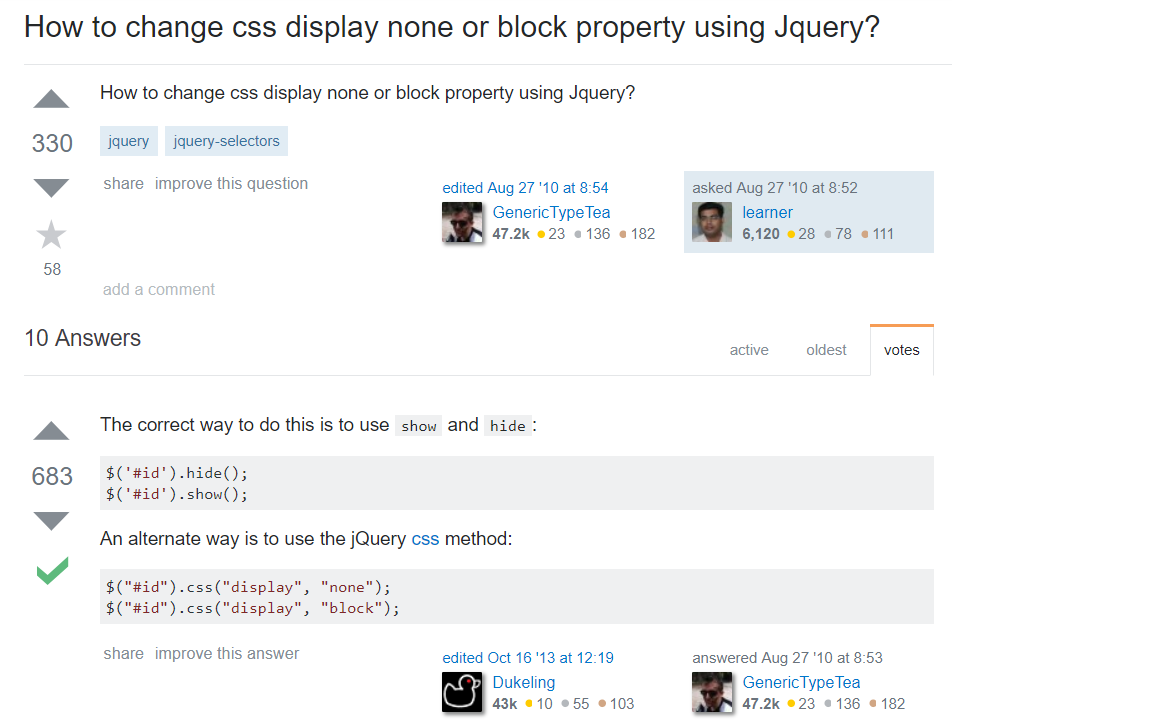
\includegraphics[width=\linewidth]{figure1.png}
  \caption{Example of an edited answer.}
  \label{fig:jqueryAnswer}
\end{figure}

Figure \ref{fig:jqueryAnswer} shows an example of an edited answer% 
\footnote{\url{https://stackoverflow.com/questions/3582619/how-to-change-css-display-none-or-block-property-using-jquery/3582629#3582629}}. 
The original author only provided one feasible and actually inferior solution, which is later complemented by a trusted community member. 
This example demonstrated a common scenario when an alternative API usage is added.

\begin{figure}
  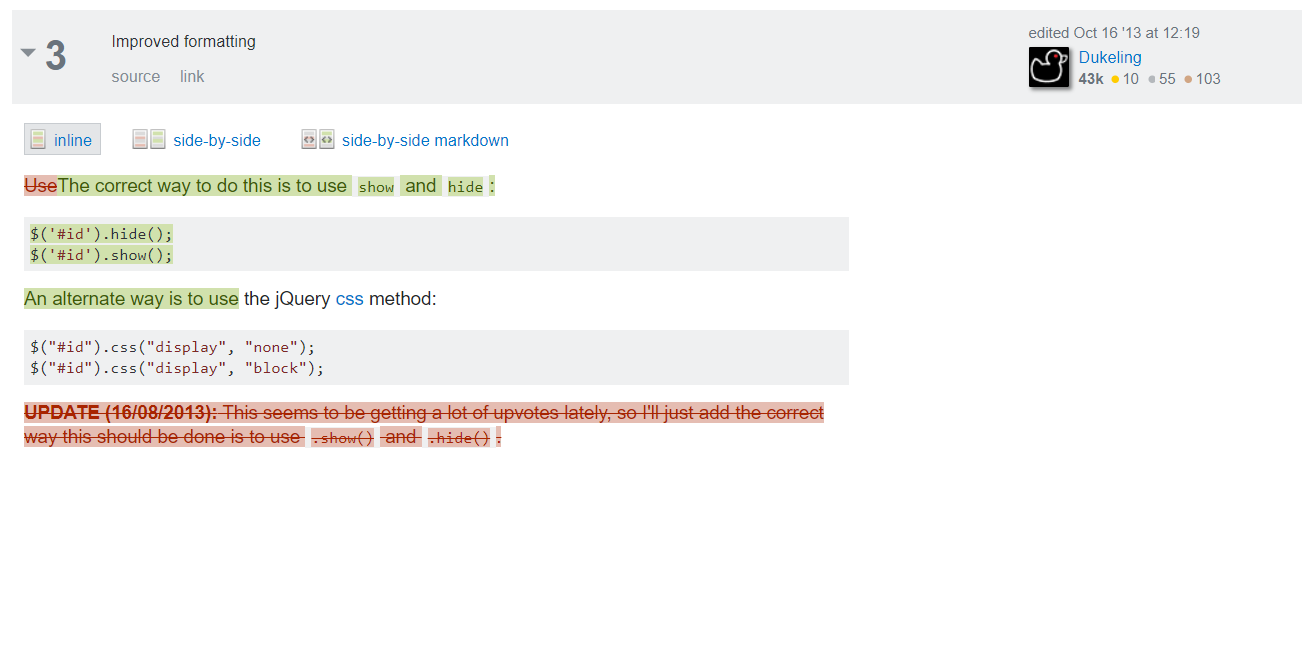
\includegraphics[width=\linewidth]{figure2.png}
  \caption{Example of a revision history record.}
  \label{fig:jqueryAnswerRevision}
\end{figure}

Additionally, the revision history of the above example is shown in Figure \ref{fig:jqueryAnswerRevision}. 
An edit summary, all modified content, the edit time, and the editor information are included in this record. 
Added content is marked green while the deleted is marked red. 
Note that the editor concluded his contribution as improving format while he actually added a whole block of information, which brings difficulty to mine the root cause of a revision. 
However, we do not have this issue since we take a manual approach to label root cause.

An answer could be edited due to various reasons, and there is an official list enumerating them \footnote{https://stackoverflow.com/help/editing} : 1) fixing grammar and spelling mistakes, 2) clarifying meaning of the post, 3) including information found only in comments, 4) correcting mistakes or adding updates, and 5) adding related resources. 
This list only provides a general overview of all editing causes, and thus not very meaningful. 
For example, an answerer could barely get any useful insight from this list to help elaborate his answer, especially when there is no comment yet.

To the best of our knowledge, no existing research investigates the completeness of answers on Stack Overflow. 
Such knowledge is useful because, for answerers it could help them compose a post that is more likely to get upvoted, and for editors it could provide them confidence for editing. 
Moreover, such knowledge can be used to detect incomplete yet accepted answers to call for improvement. 
All these implications can in turn improve the overall quality of this community and thus help its countless users.

\jyy{I think the word ``complete'' itself may need more explanations. Should a complete answer involve \emph{anything} needed to understand related issues? (E.g., the CSS display in the motivating example.). I feel that should be included is certainly subjective, and there is trade-off between brevity, the relevance to the question, etc. An overly complete answer maybe very difficult to read.}

\gz{ Compared with the completeness of documentation, the completeness of an answer can be easier to define (in a relative and coarse manner, which sounds a bit sneaky):

Let {\em q} be a question of type {\em qi}, which is from the prescribed question types 
\{q1, q2, ..., qn\}, and let {\em ai} be the prescribed(mined) set of answer components ever appeared under {\em qi}. Let {\em a} be an answer of {\em q}. Then {\em a} is complete when the set of sentences {\em s} in {\em a} covered each component in {\em ai}.  

The better we define question types and answer components, the more sense this definition will make.

For your question on the motiving example, notice the asker already confines his "expected output" to a technical detail(css display: none or block), and therefore we can infer no more information on css display is needed. On the other hand, since he asked how to do it with {\em jQuery}, alternative API usages should be given in a comprehensive manner.  

Then, for our experiment part, we(me) want to devise a static analysis chrome extension to analyse question properties to categorize question and then inform our answerer of what kind of information will be useful to add in the answer, to this specific type of question, and ideally provides some example pieces from the best typical answers. Personally, as a newcomer in the community who is learning the community norm, and need some accepted answers to encourage himself, I think such tool is tremendously useful. This task is technically challenging and I'm curious to see how far we can go (how much constraint we eventually have to create to narrow down to a solvable degree).

To evaluate the tool, email-spam some unlucky guys to ask for feedback.

As for the readability issue, I think answerer could put worked solution upfront(TL;DR), followed with explanation and links. It sounds like a HCI problem, and I guess it's not a big issue, huh?}

One may argue that an answer does not have to be complete, as long as the asker finds it helpful. 
However, Stack Overflow has been a primary learning resource for many programmers \footnote{https://insights.stackoverflow.com/survey/2018/\#technology}, and thus each answer can potentially influence gazillions of programmers who may visit the same page with various background and problem contexts. 
Without the consideration of its vast audience, an answer can have horrifying ramification. 
For example, a tailored insecure code snippet without noticeable warning could be copied and used in hundreds of thousands of applications \cite{DBLP:conf/sp/FischerBXSA0F17}, raising big security concern. 

\jyy{From the argument, I can't imply that answers should be complete. Still, I'm convinced that there must be some fundamental issues to be addressed or clarified to make an answer good. Maybe we can focus on the research of revision history itself, and propose some interesting findings.}

\gz { Then I will try harder to convince you. Here are other possible antitheses of completeness on answers:

1. "People only read what they want to read and additional information just eludes their eyes." 

My defense: addtional information adds an air of authority and eases the persuasion; not everyone comes to the answer in a hurry only for the worked solution, some may want to learn more and read the answers all. Similar to the fact that we have both good students and bad students.  

2. "Comprehensive information is useless. Why should I know alternative ways to hide a \<div\>? One worked solution is enough for me."

My defense: to answer job interview questions like how many ways are there in JavaScript to bind 'this', and all the rationale behind this type of interview question. Why don't programmers learn them from books and documentation? They said good programmers only learn in practice, and asking stack overflow is a typical phase in practice.

3. "It sounds too restricted and unnatural. Why should an answerer be prohibited from freely expressing himself?"

My defense: Stack Overflow has its own vision to become the structured and objective knowledgebase of programming, and it explicitly discourages traditional carefree conversation. If one still favors free discussion, the comment area is for him. (Think of the answer as a serious pull request to the issue, and comments are like comments on GitHub)

Ideally, I shall add these discussions to this paper and find some empirical study to back up my statements. That's a lot of time.

}

\section {Research questions}
\begin{itemize}
  \item RQ1. What types of information may get added to an answer after it's been 1) posted 2) accepted, and what is their relation with the question type, if there is any?
  \item RQ2. How long does it take the community to fill each type of missing information?
  \item RQ3. Who is more likely to augment each type of information?
\end{itemize}

\jyy{It looks very good to decompose a StackOverflow answer into components (examples, links, references, patterns/antipatterns, ...). Is this idea new or someone already did the study? If not (or you're not satisfied with the related work), it worths a careful study as a research question: what may appear in an answer?}

\jyy{Then, a (maybe large) quantitative analysis to the revision history can be conducted based on seeing what components are frequently added/revised in the revision history. This process is highly non-trivial and will support your later findings.}

\jyy{Then many other questions can be answered with the previous results: who is likely to augment information, what makes an answer great, etc.}

\gz { The most comprehensive work on this decomposed answers into Explanation, Source Code, Redirecting, Clue/Hint/Suggestion, Alternative, Tutorial, Announcement, Opinion(which shouldn't appear actually), and Benchmark. 

Existing categorization didn't consider the relation between question and answer, e.g. the above work only independently analyzed what information is in questions and what is in answers, since they focused on more holistical view on community

I can use the projector to show you a table listing related study}

{\em Proposition1} 
Alternative API usage, insertion to correct API misuse, links of references, links to learning resources, code example to demonstrate approachs, warning for when this solution may not apply, warning for non-functional issue of this solution, surrouding text or code comments explaining what the code does, and complete instructions on how to use the code may get added to an answer. 
Common missing types may be different within different question types, and the latter is previously conclude as 1) Looking for help with debugging, 2) Asking the capability of certain technology, 3) Eliciting implementation for a given task, and 4) Seeking alternative solution. \cite{DBLP:conf/icsm/NasehiSMB12}   

{\em Proposition2}
NaN.

{\em Proposition3}
Warnings are more likely to be added by other collaborators, while comments and surrouding text are typically augmented by the original author. 



\section {Data Collection and Analysis}
We can download Stack Overflow data dump \footnote{https://archive.org/download/stackexchange} which contains all questions, answers, comments as well as their respective revision histories from 2007 to June 2018. 
This dataset serves as our main data source.

\subsection {Definition of the Augmentation}
In the above dataset, revision record is in the form of markdown-based or html-based full string. 
Inspired by a mining work from Baltes et al. \cite{DBLP:journals/corr/abs-1803-07311}, we define each element in markdown or HTML as a block. 
Additionally, we extract each line comment within a code block as an individual block. 
An edit may insert a new block or delete existing block (note we consider a update as an addition of one insertion and one deletion). 
We define an augmentation record as an edit only inserting new blocks. 
\jyy{Study only augmentations may have threats. You may carefully think about it.}


\subsection {Process}
We only select posts with the tag of javascript as a representation. 
We believe posts revolving javascript is representative enough since javascript, as the most popular language both in terms of the post numbers within the community, has been used in many domains. 
We further filter the revision history dataset, only saving augmentation record.

Then, from the dataset, we first randomly sample 50 accepted answers with augmentation record and over 100 upvotes, construct the initial missing types based on their records as well as our own experience.\jyy{We may have some further discussions on this.}

After that, we randomly select 400 more accepted answers without upvoting constraint. 
We manually inspect their type and iteratively refine our model. 
After this process, we get a dataset of 400+ augmentation record each labelled with 1) corresponding missing types, 2) edited time, 3) answered time of the original answer, 4) accepted time of the answer, 5) question type, and 6) whether the editor is the original author, or a trusted contributor, or a novice.

Then we can handily answer each of our research questions.

\section {Related work}

\jyy{I think you have already collected strongly-related work. If you have time, you can read them and find which relevant papers are cited by them. Generally we'd have 30-40 citations, and less relevant work can be just mentioned in our related work.}

\subsection {Revisions on Stack Overflow}

Li et al. \cite{JIT1397} trained a classfier to predict whether a post should be edited. 
They didn't qualitatively investigate the root cause of edits. 
(Note I can't get access to this paper and thus didn't actually read it)

Chen et al. \cite{Chen:2017:CCD:3171581.3134667} devised a RNN model to correct domain-related sentences, but they only addressed syntactic issues. 
They also conducted a study on the nature of the root cause of edits, nevertheless, they used the same catogary model as the official list, which is vague on its own.

Li et al. \cite{7208aa781175403f9c3aaddc19f3b8cf} confirmed the success of introducing such revision system to Stack Overflow with the finding that the improved content quality overweighs the reduced incentives to contribute. 
Our work could further the flourishing of this community by helping answerers understand when and why their answer should be revised and thus decrease the likelyhood that they feel discouraged after their answers are edited. 

Baltes et al. \cite{DBLP:journals/corr/abs-1803-07311} briefly investigated the characteristic of an edited post, and they found the posts with more edits tend to have more comments.  

None of the above work conducted in-depth qualitative study on what types of information may get added by edits. 

\subsection {Answer Quality Evaluation}

The Information Retrieval community has taken various statistical approaches to rank answer wrt quality in community-based QA (CQA) systems. \cite{DBLP:journals/corr/SugguGCS16, Dalip:2013:EUF:2484028.2484072, Shah:2010:EPA:1835449.1835518, 7857066} They have developed a rich set of multi-level features to predict answer quality, from the answer itself to its parental question and finally their general category, covering both textual features and non-textual ones. 
These work have two big limitations: first, they cannot explain how and why each feature contributes to the final quality and thus cannot help revise an answer, second, since they are mainly focused on general CQA system, domain-specific community like Stack Overflow needs more insights to build a professional quality standard.    

To enable people to jointly leverage features of both questions and answers from Stack Overflow, Yao et al. \cite{DBLP:journals/corr/YaoTXAXL13} proposed a framework for statistical prediction task, the features used in which can be independently input by framework users. 
They only conducted a small study on the quality correlation between an answer and its question in terms of their received votes.  

The work from Nasehi et al. \cite{DBLP:conf/icsm/NasehiSMB12} is closest to ours. 
They studied the charactertistics of good code examples from highly-voted answers on Stack Overflow, and found that good code examples leave out irrelevant details, make use of context that is familiar to the asker, highlight important content, contain step-wise explanation, and provide resource links. 
They also found bad answers lack necessary code as well as statement of their limitation. 
Compared with their work, we dig into the history of good answers, and try to understand what answerers often miss when they first pose an answer and how difficult it is to have someone fix it. 
With such insight, we can further identify the greatest scarcity of knowledge within the community and in turn take some actions, e.g. revise the reputation system to reflect and attract rare expertise.      

\section {Threats to Validity}
Not all programmers use Stack Overflow, and not all of its users have answered or edited answers. 
Those who augmented an answer may only add what they think is necessary, deviating from what most programmers expect for a complete answer. 
We recognize and admit this as an external validity threat. 

Additionally, there may exist significant difference between answers for different programming language. 
However, we (may) find our conceptual model constructed from javascript-related answers rather universal.

Moreover, we use average needed time to get complemented for each type of missing information to reflect scarcity of different knowledge in the community, but our sample is rather limited to be generalizable to the whole community. 


\jyy{If a cited paper is published, you'd better cite the conference/journal version instead of the arxiv version. Please check if there're such cases.}

\gz{ SOTorrent[5] is published in MSR 2018 which doesn't have public bibtex yet; Deep feature fusion[7] is a SIGIR workshop paper which didn't have a formal citation entry; "Want a good answer?"[11] is not published. Maybe I shall consider deleting some of them and switch to published work.}

\bibliographystyle{unsrt}
\bibliography{references}

\end{document}




